% Capítulo 5 (Metodologia) — Slide 0 — Pipeline de evidência do AIPE (síntese, figura isolada)
\begin{frame}{Síntese do pipeline metodológico}
  \centering
  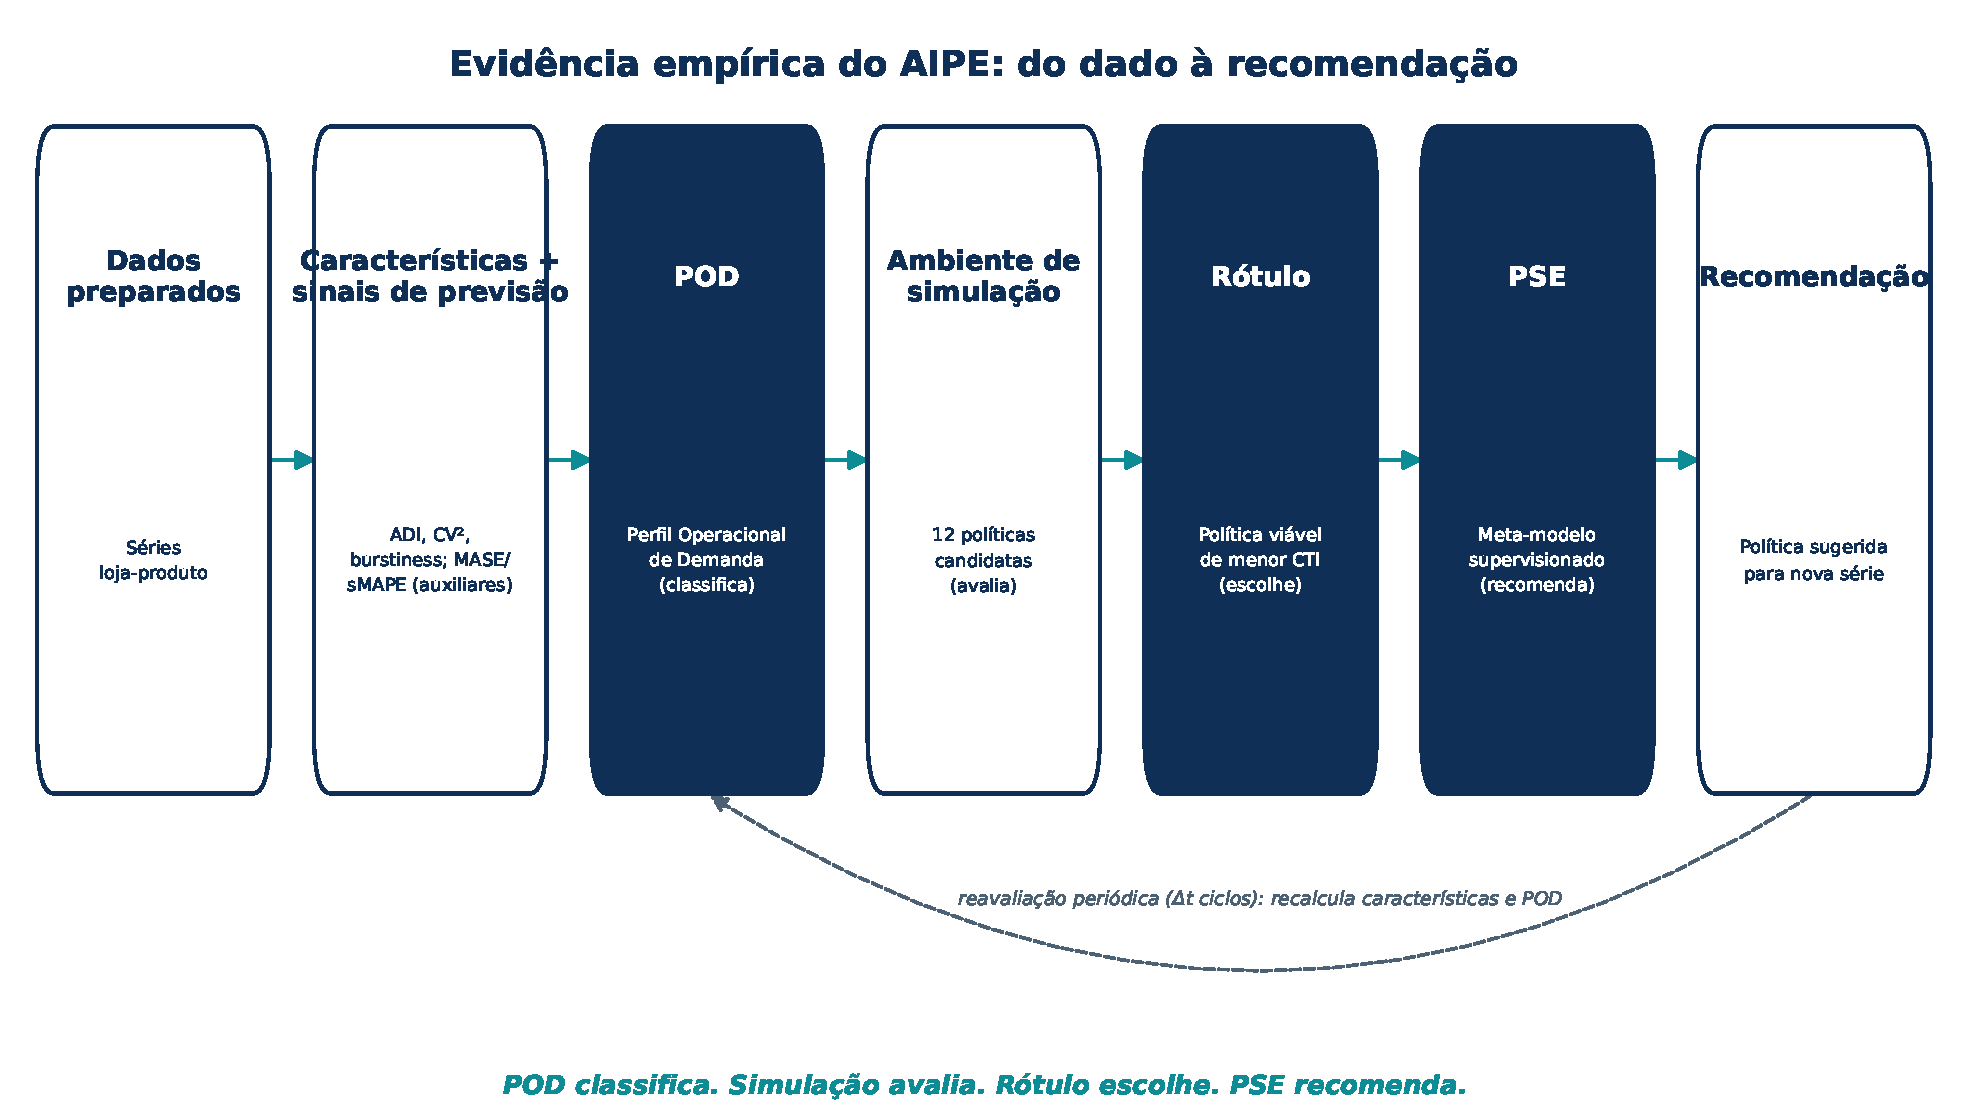
\includegraphics[width=\linewidth,height=6.5cm,keepaspectratio]{figures/aipe_evidence_pipeline.pdf}
  \note{
    Esta figura sintetiza a metodologia que será detalhada nos próximos
    slides. A leitura é sempre a mesma, da esquerda para a direita: o POD
    classifica a série em um perfil operacional; o ambiente de simulação
    avalia as 12 políticas candidatas sob as mesmas condições; o rótulo
    escolhe, entre as políticas viáveis (NS $\geq$ 0,70), a de menor CTI; e o
    PSE aprende essa relação entre características e rótulo, para depois
    recomendar uma política a novas séries. Note que cada etapa tem um verbo
    diferente -- classifica, avalia, escolhe, aprende/recomenda -- porque
    cada uma tem uma responsabilidade distinta: o POD não escolhe a
    política, e o PSE não gera o rótulo, ele aprende a partir dele.
  }
\end{frame}
